\documentclass[12pt,a4paper]{article}
\usepackage{cite}
\usepackage{amsmath}
\usepackage{graphicx}
\usepackage{booktabs}
\usepackage{multirow}
\usepackage{url}
\usepackage{array}
\usepackage{float}
\usepackage{xcolor}
\usepackage{geometry}
\usepackage{setspace}
\usepackage{titlesec}

\geometry{a4paper, margin=1in}
\setstretch{1.15}
\setlength{\parindent}{0pt}
\setlength{\parskip}{6pt}

\title{Comparative Evaluation of Machine Learning Models for Diabetes Status Prediction Using the Pima Indians Diabetes Dataset}

\author{
\begin{tabular}{ccc}
Author 1 & Author 2 & Author 3 \\
Author 4 & Author 5 & Author 6 \\
Author 7 & Author 8 & Author 9
\end{tabular}\\[1em]
Department of Computer Science and Engineering\\
GITAM (Deemed to be University)
}
\date{}

\begin{document}
\maketitle
\thispagestyle{empty}
\clearpage

\begin{abstract}
Diabetes status prediction using routinely recorded clinical measurements is a common machine-learning classification task. This study compares Logistic Regression, Decision Tree, and Random Forest classifiers using the Pima Indians Diabetes dataset, which contains 768 records and eight predictor variables. Implausible zero values in five measurement columns were treated as missing, with median imputation performed within model pipelines to avoid using test-set information during preprocessing. The data were divided into stratified training and test subsets using an 80:20 split. Baseline models were evaluated using accuracy, precision, recall, F1-score, and ROC-AUC. Five-fold cross-validation and grid-search hyperparameter tuning were conducted on the training subset, and a separate held-out test subset was used for final evaluation. On the test set, the baseline Decision Tree achieved the highest accuracy (79.2\%) and F1-score (70.9\%), while the baseline Random Forest achieved the highest ROC-AUC (0.817). After tuning for cross-validation F1-score, Random Forest obtained the highest test recall (74.1\%) and F1-score (66.1\%) among the tuned models, although its accuracy was 73.4\%. Feature selection using the five highest ANOVA F-score features produced model-dependent effects rather than consistent improvements. Permutation importance identified Glucose, BMI, and Age as the leading features for the baseline Random Forest. The findings demonstrate the importance of evaluating multiple metrics and separating model selection from final testing. The dataset is limited to a specific population and records diabetes status rather than time to disease onset; therefore, the results should not be interpreted as evidence of prospective early diagnosis or clinical readiness.
\end{abstract}

\noindent\textbf{Keywords:} Diabetes status prediction, machine learning, Logistic Regression, Decision Tree, Random Forest, feature selection, hyperparameter tuning, Pima Indians Diabetes Dataset.

\clearpage
\section{Introduction}
Diabetes mellitus is a major chronic health condition, and data-driven methods have been investigated to support classification and risk assessment. Machine-learning approaches can learn patterns from clinical measurements, but their performance depends on data quality, evaluation design, population characteristics, and the metric used to assess predictions. A systematic review by Chaki \textit{et al.} discusses the use of machine learning and artificial intelligence across diabetes detection, diagnosis, preprocessing, feature selection, and performance assessment \cite{chaki2022}. Research has also examined the Pima Indians Diabetes dataset using a range of classifiers, including interpretable models and ensemble methods \cite{naz2020,chang2023}.

This study conducts a controlled comparison of three commonly used classifiers: Logistic Regression, Decision Tree, and Random Forest. In addition to baseline evaluation, the study investigates whether hyperparameter tuning and reducing the feature set from eight variables to five affect predictive performance. Permutation importance is used to describe how the selected baseline model relies on individual input variables.

The contributions of this work are:
\begin{itemize}
    \item a reproducible preprocessing and evaluation workflow with median imputation inside model pipelines;
    \item a comparison of baseline and hyperparameter-tuned classifiers using multiple evaluation metrics;
    \item an experiment comparing all eight predictors with five features selected using ANOVA F-scores; and
    \item a model-agnostic permutation-importance analysis of the baseline model with the highest test ROC-AUC.
\end{itemize}

The term \emph{diabetes status prediction} is used throughout this paper. The available dataset contains a binary outcome label and does not provide a prospective time-to-onset target. Accordingly, this experiment does not establish the ability to detect diabetes before its onset.

\clearpage
\section{Related Work}
Smith \textit{et al.} introduced the ADAP learning algorithm in work on forecasting diabetes onset using data associated with the Pima population \cite{smith1988}. Subsequent research has continued to use this dataset to compare machine-learning classifiers. Naz and Ahuja explored a deep-learning approach for diabetes prediction using the Pima dataset \cite{naz2020}. Chang \textit{et al.} compared interpretable supervised learning methods, including Naive Bayes, Random Forest, and a decision-tree model, and discussed the role of feature selection and model interpretability \cite{chang2023}.

Chaki \textit{et al.} reviewed machine-learning and artificial-intelligence approaches for diabetes detection and self-management, covering datasets, preprocessing, feature selection, classification techniques, and performance measures \cite{chaki2022}. These studies motivate evaluating not only a single accuracy value but also precision, recall, F1-score, and ROC-AUC. The present work is a small comparative experiment on one public dataset; it is not a direct replication of the methods or results of the cited studies.

\clearpage
\section{Dataset Description}
The experiment uses the \emph{diabetes.csv} file obtained from the Kaggle dataset page supplied for this project \cite{kagglepima}. The dataset contains 768 observations, eight predictor variables, and one binary target variable named \texttt{Outcome}. The commonly documented Pima dataset contains adult women of Pima heritage, and its population scope limits generalisation to other demographic groups \cite{pimaRdoc}.

The input variables are Pregnancies, Glucose, BloodPressure, SkinThickness, Insulin, BMI, DiabetesPedigreeFunction, and Age. The target is \texttt{Outcome}, where 0 denotes no recorded diabetes and 1 denotes recorded diabetes in the dataset. The class distribution is 500 records (65.1\%) for class 0 and 268 records (34.9\%) for class 1.

\begin{figure}[t]
\centering
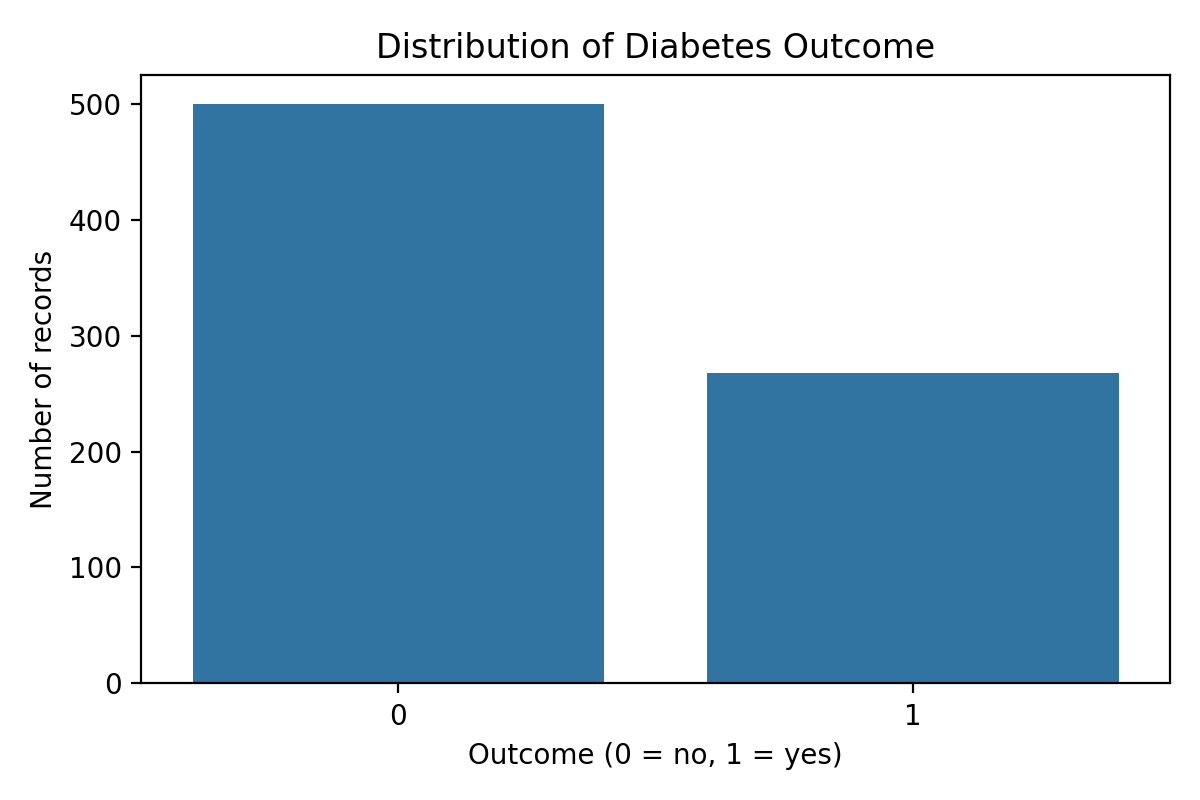
\includegraphics[width=\columnwidth]{figures/outcome_distribution.png}
\caption{Distribution of the binary outcome in the dataset.}
\label{fig:outcome}
\end{figure}

\begin{table}[t]
\caption{Dataset Summary}
\label{tab:dataset}
\centering
\begin{tabular}{lr}
\toprule
Property & Value\\
\midrule
Observations & 768\\
Predictor variables & 8\\
Target variable & Outcome\\
Class 0 & 500 (65.1\%)\\
Class 1 & 268 (34.9\%)\\
Training observations & 614\\
Test observations & 154\\
Train/test ratio & 80:20\\
\bottomrule
\end{tabular}
\end{table}

\clearpage
\section{Methodology}
\subsection{Data Cleaning and Preprocessing}
The notebook identified zero values in Glucose (5), BloodPressure (35), SkinThickness (227), Insulin (374), and BMI (11). These values were treated as implausible missing measurements and converted to NaN. Zero values in Pregnancies were retained because they can be valid. No duplicate rows were reported.

Missing values were imputed using the median through \texttt{SimpleImputer} inside each machine-learning pipeline. Consequently, the imputation statistics were learned from the training data within each fit and then applied to the corresponding validation or test data. StandardScaler was included in the Logistic Regression pipeline; the Decision Tree and Random Forest pipelines did not include scaling.

\subsection{Train--Test Split}
The data were split into 80\% training and 20\% test subsets using stratification on the target variable and random state 42. This produced 614 training records and 154 test records. The positive-class proportions were approximately 34.9\% in the training set and 35.1\% in the test set.

\subsection{Baseline Classifiers}
Three classifiers were evaluated:
\begin{itemize}
    \item \textbf{Logistic Regression:} fitted with a maximum of 2000 iterations and random state 42, preceded by median imputation and standardisation.
    \item \textbf{Decision Tree:} configured with maximum depth 4 and minimum leaf size 10, preceded by median imputation.
    \item \textbf{Random Forest:} configured with 300 trees, minimum leaf size 5, and balanced class weights, preceded by median imputation.
\end{itemize}

\subsection{Hyperparameter Tuning}
GridSearchCV was applied separately to each classifier using five-fold stratified cross-validation on the training subset. The search evaluated multiple parameter combinations, with the parameter grids specified in the accompanying notebook. Accuracy, precision, recall, F1-score, and ROC-AUC were recorded during cross-validation. The refit metric was F1-score. The best estimator from each search was then evaluated on the held-out test set. The test set was not used to select hyperparameters.

\subsection{Feature Selection}
SelectKBest with the ANOVA F-test (\texttt{f\_classif}) was used to select five features from the original eight. The selector was placed inside each model pipeline so that feature selection was fitted using training data only. The selected feature set was Glucose, SkinThickness, Insulin, BMI, and Age for all three classifiers in this run.

\subsection{Permutation Importance}
Permutation importance was computed for the baseline model with the highest test ROC-AUC. Each feature was shuffled repeatedly, and the resulting decrease in ROC-AUC was used as the importance measure. Twenty repeats were used with random state 42. Importance is interpreted as model reliance in this dataset and split, not as causal evidence.

\subsection{Evaluation Metrics}
The study reports accuracy, precision, recall, F1-score, and ROC-AUC. For the positive class, precision measures the proportion of positive predictions that were correct, while recall measures the proportion of recorded positive cases identified by the classifier. F1-score is the harmonic mean of precision and recall. ROC-AUC measures ranking discrimination across classification thresholds. No single metric is treated as sufficient on its own.

\clearpage
\section{Experimental Results}
\subsection{Baseline Test-Set Performance}
Table~\ref{tab:baseline} presents the baseline test-set results. The Decision Tree achieved the highest accuracy (79.2\%), precision (69.6\%), recall (72.2\%), and F1-score (70.9\%). Random Forest achieved the highest ROC-AUC (0.817), followed closely by Logistic Regression (0.813). These results illustrate that the model with the highest accuracy need not have the highest ROC-AUC.

\begin{table}[t]
\caption{Baseline Performance on the Held-Out Test Set}
\label{tab:baseline}
\centering
\begin{tabular}{lccccc}
\toprule
Model & Acc. & Prec. & Rec. & F1 & AUC\\
\midrule
Logistic Regression & 0.708 & 0.600 & 0.500 & 0.545 & 0.813\\
Decision Tree & \textbf{0.792} & \textbf{0.696} & \textbf{0.722} & \textbf{0.709} & 0.801\\
Random Forest & 0.747 & 0.632 & 0.667 & 0.649 & \textbf{0.817}\\
\bottomrule
\end{tabular}
\end{table}

\begin{figure}[t]
\centering
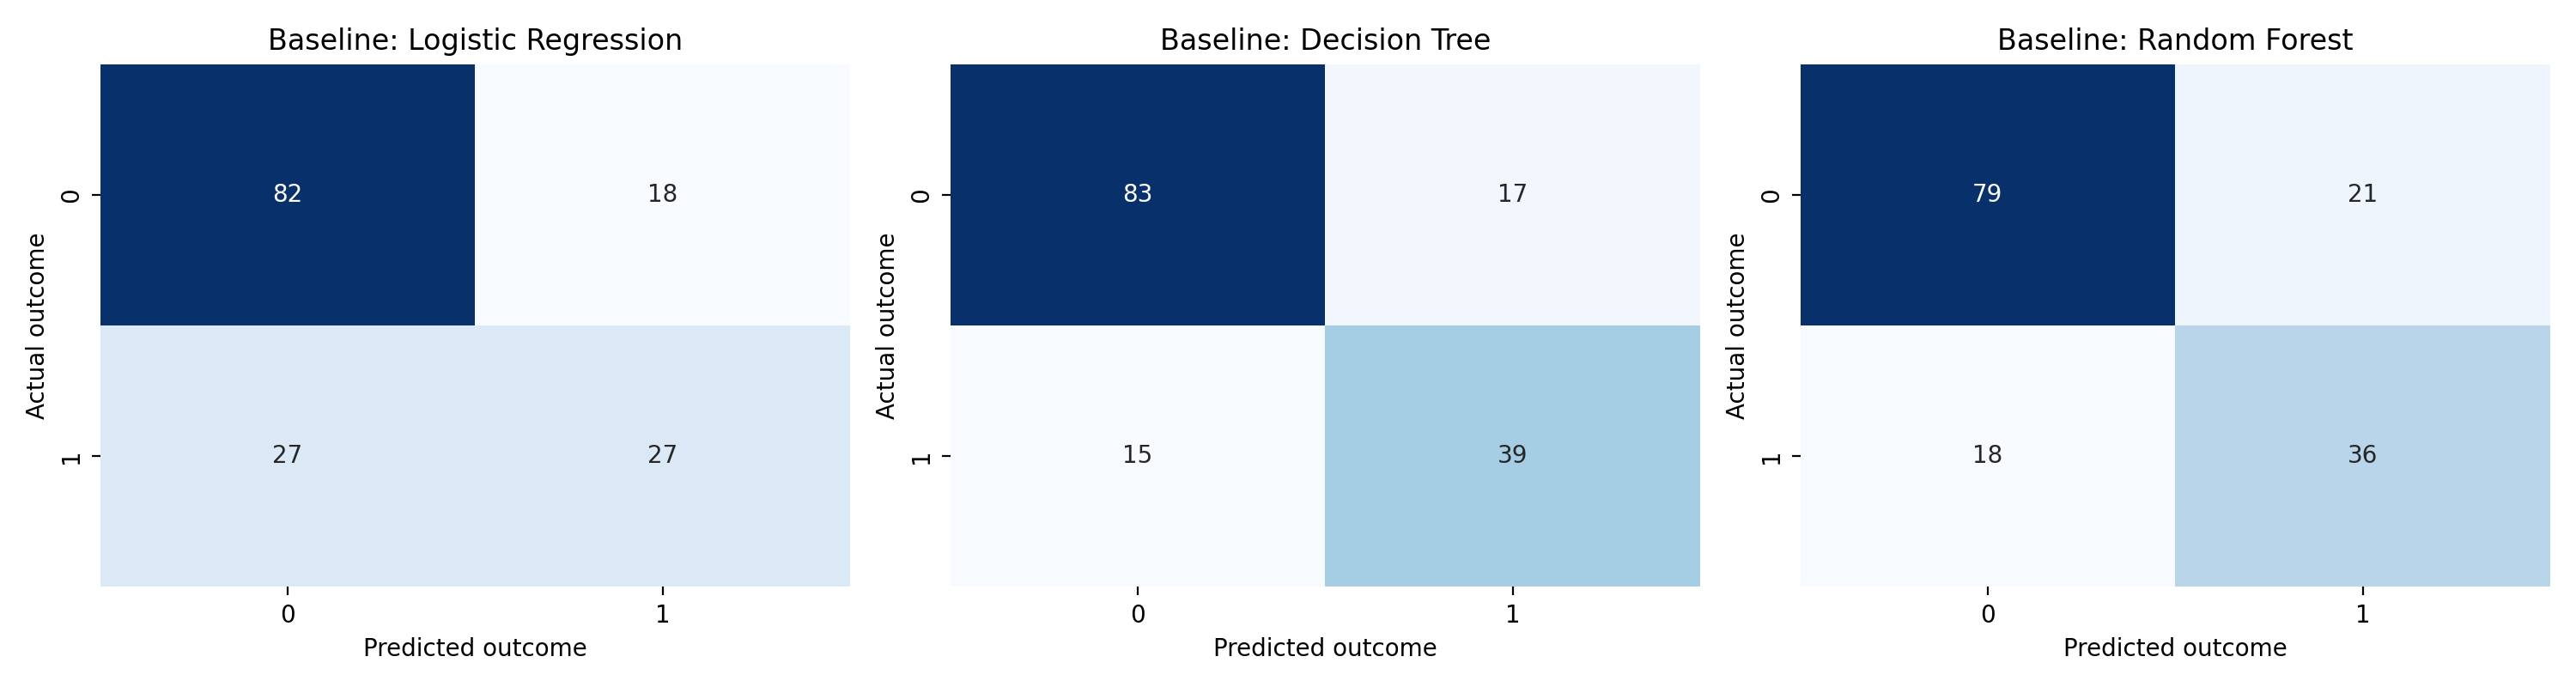
\includegraphics[width=\columnwidth]{figures/baseline_confusion_matrices.png}
\caption{Confusion matrices for the three baseline classifiers on the test set.}
\label{fig:confusion}
\end{figure}

\begin{figure}[t]
\centering
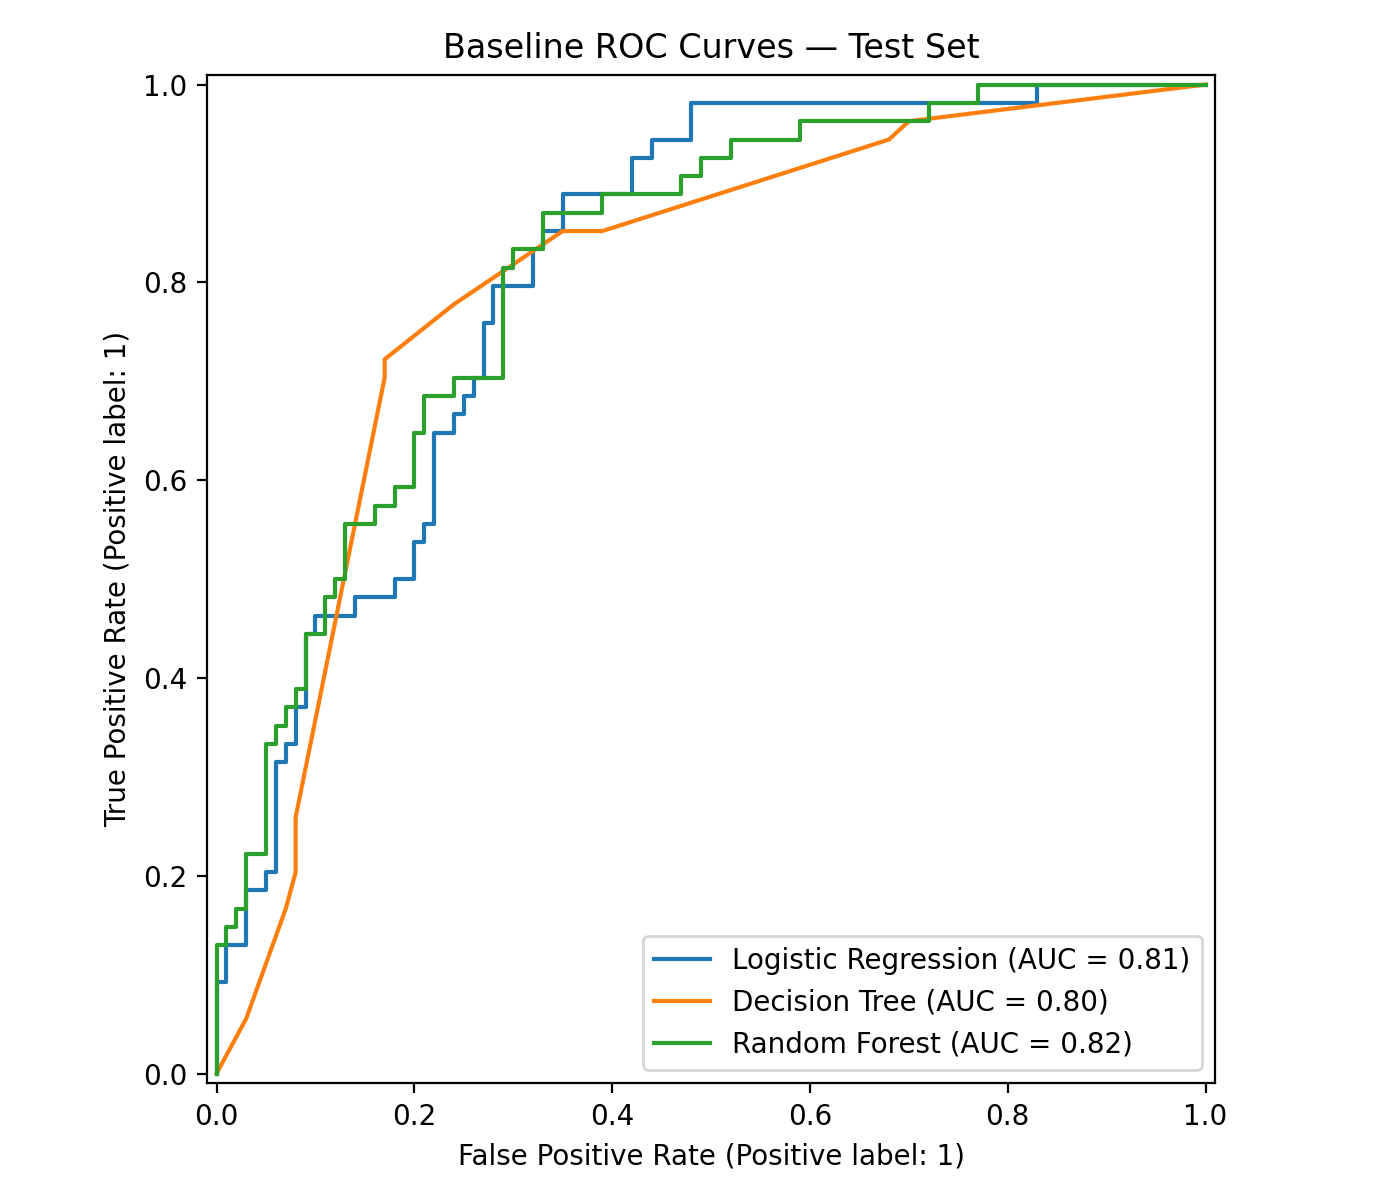
\includegraphics[width=0.9\columnwidth]{figures/baseline_roc_curves.png}
\caption{ROC curves for the baseline classifiers on the test set.}
\label{fig:roc}
\end{figure}

\subsection{Hyperparameter-Tuned Performance}
Table~\ref{tab:tuned} reports the tuned models on the held-out test set. Random Forest achieved the highest recall (0.741), F1-score (0.661), and ROC-AUC (0.820) among the tuned models. Logistic Regression achieved an F1-score of 0.615 and ROC-AUC of 0.810. The tuned Decision Tree recorded an accuracy of 0.727 and ROC-AUC of 0.771.

\begin{table}[t]
\caption{Tuned Model Performance on the Held-Out Test Set}
\label{tab:tuned}
\centering
\begin{tabular}{lccccc}
\toprule
Model & Acc. & Prec. & Rec. & F1 & AUC\\
\midrule
Logistic Regression & 0.708 & 0.571 & 0.667 & 0.615 & 0.810\\
Decision Tree & 0.727 & 0.611 & 0.611 & 0.611 & 0.771\\
Random Forest & 0.734 & 0.597 & \textbf{0.741} & \textbf{0.661} & \textbf{0.820}\\
\bottomrule
\end{tabular}
\end{table}

\subsection{Baseline--Tuned Comparison}
The comparison in Table~\ref{tab:comparison} shows that tuning produced metric-dependent changes. For Random Forest, test recall increased from 0.667 to 0.741 and F1-score increased from 0.649 to 0.661, while accuracy decreased from 0.747 to 0.734 and precision decreased from 0.632 to 0.597. For Logistic Regression, recall increased from 0.500 to 0.667 and F1-score increased from 0.545 to 0.615, while precision decreased from 0.600 to 0.571. Decision Tree performance decreased across all reported test metrics after tuning. Thus, tuning did not uniformly improve all models or metrics.

\begin{table}[t]
\caption{Baseline Versus Tuned Test-Set Results}
\label{tab:comparison}
\centering
\begin{tabular}{llcc}
\toprule
Model & Metric & Baseline & Tuned\\
\midrule
\multirow{5}{*}{Logistic Regression}
& Accuracy & 0.708 & 0.708\\
& Precision & 0.600 & 0.571\\
& Recall & 0.500 & 0.667\\
& F1-score & 0.545 & 0.615\\
& ROC-AUC & 0.813 & 0.810\\
\midrule
\multirow{5}{*}{Decision Tree}
& Accuracy & 0.792 & 0.727\\
& Precision & 0.696 & 0.611\\
& Recall & 0.722 & 0.611\\
& F1-score & 0.709 & 0.611\\
& ROC-AUC & 0.801 & 0.771\\
\midrule
\multirow{5}{*}{Random Forest}
& Accuracy & 0.747 & 0.734\\
& Precision & 0.632 & 0.597\\
& Recall & 0.667 & 0.741\\
& F1-score & 0.649 & 0.661\\
& ROC-AUC & 0.817 & 0.820\\
\bottomrule
\end{tabular}
\end{table}

\begin{figure}[t]
\centering
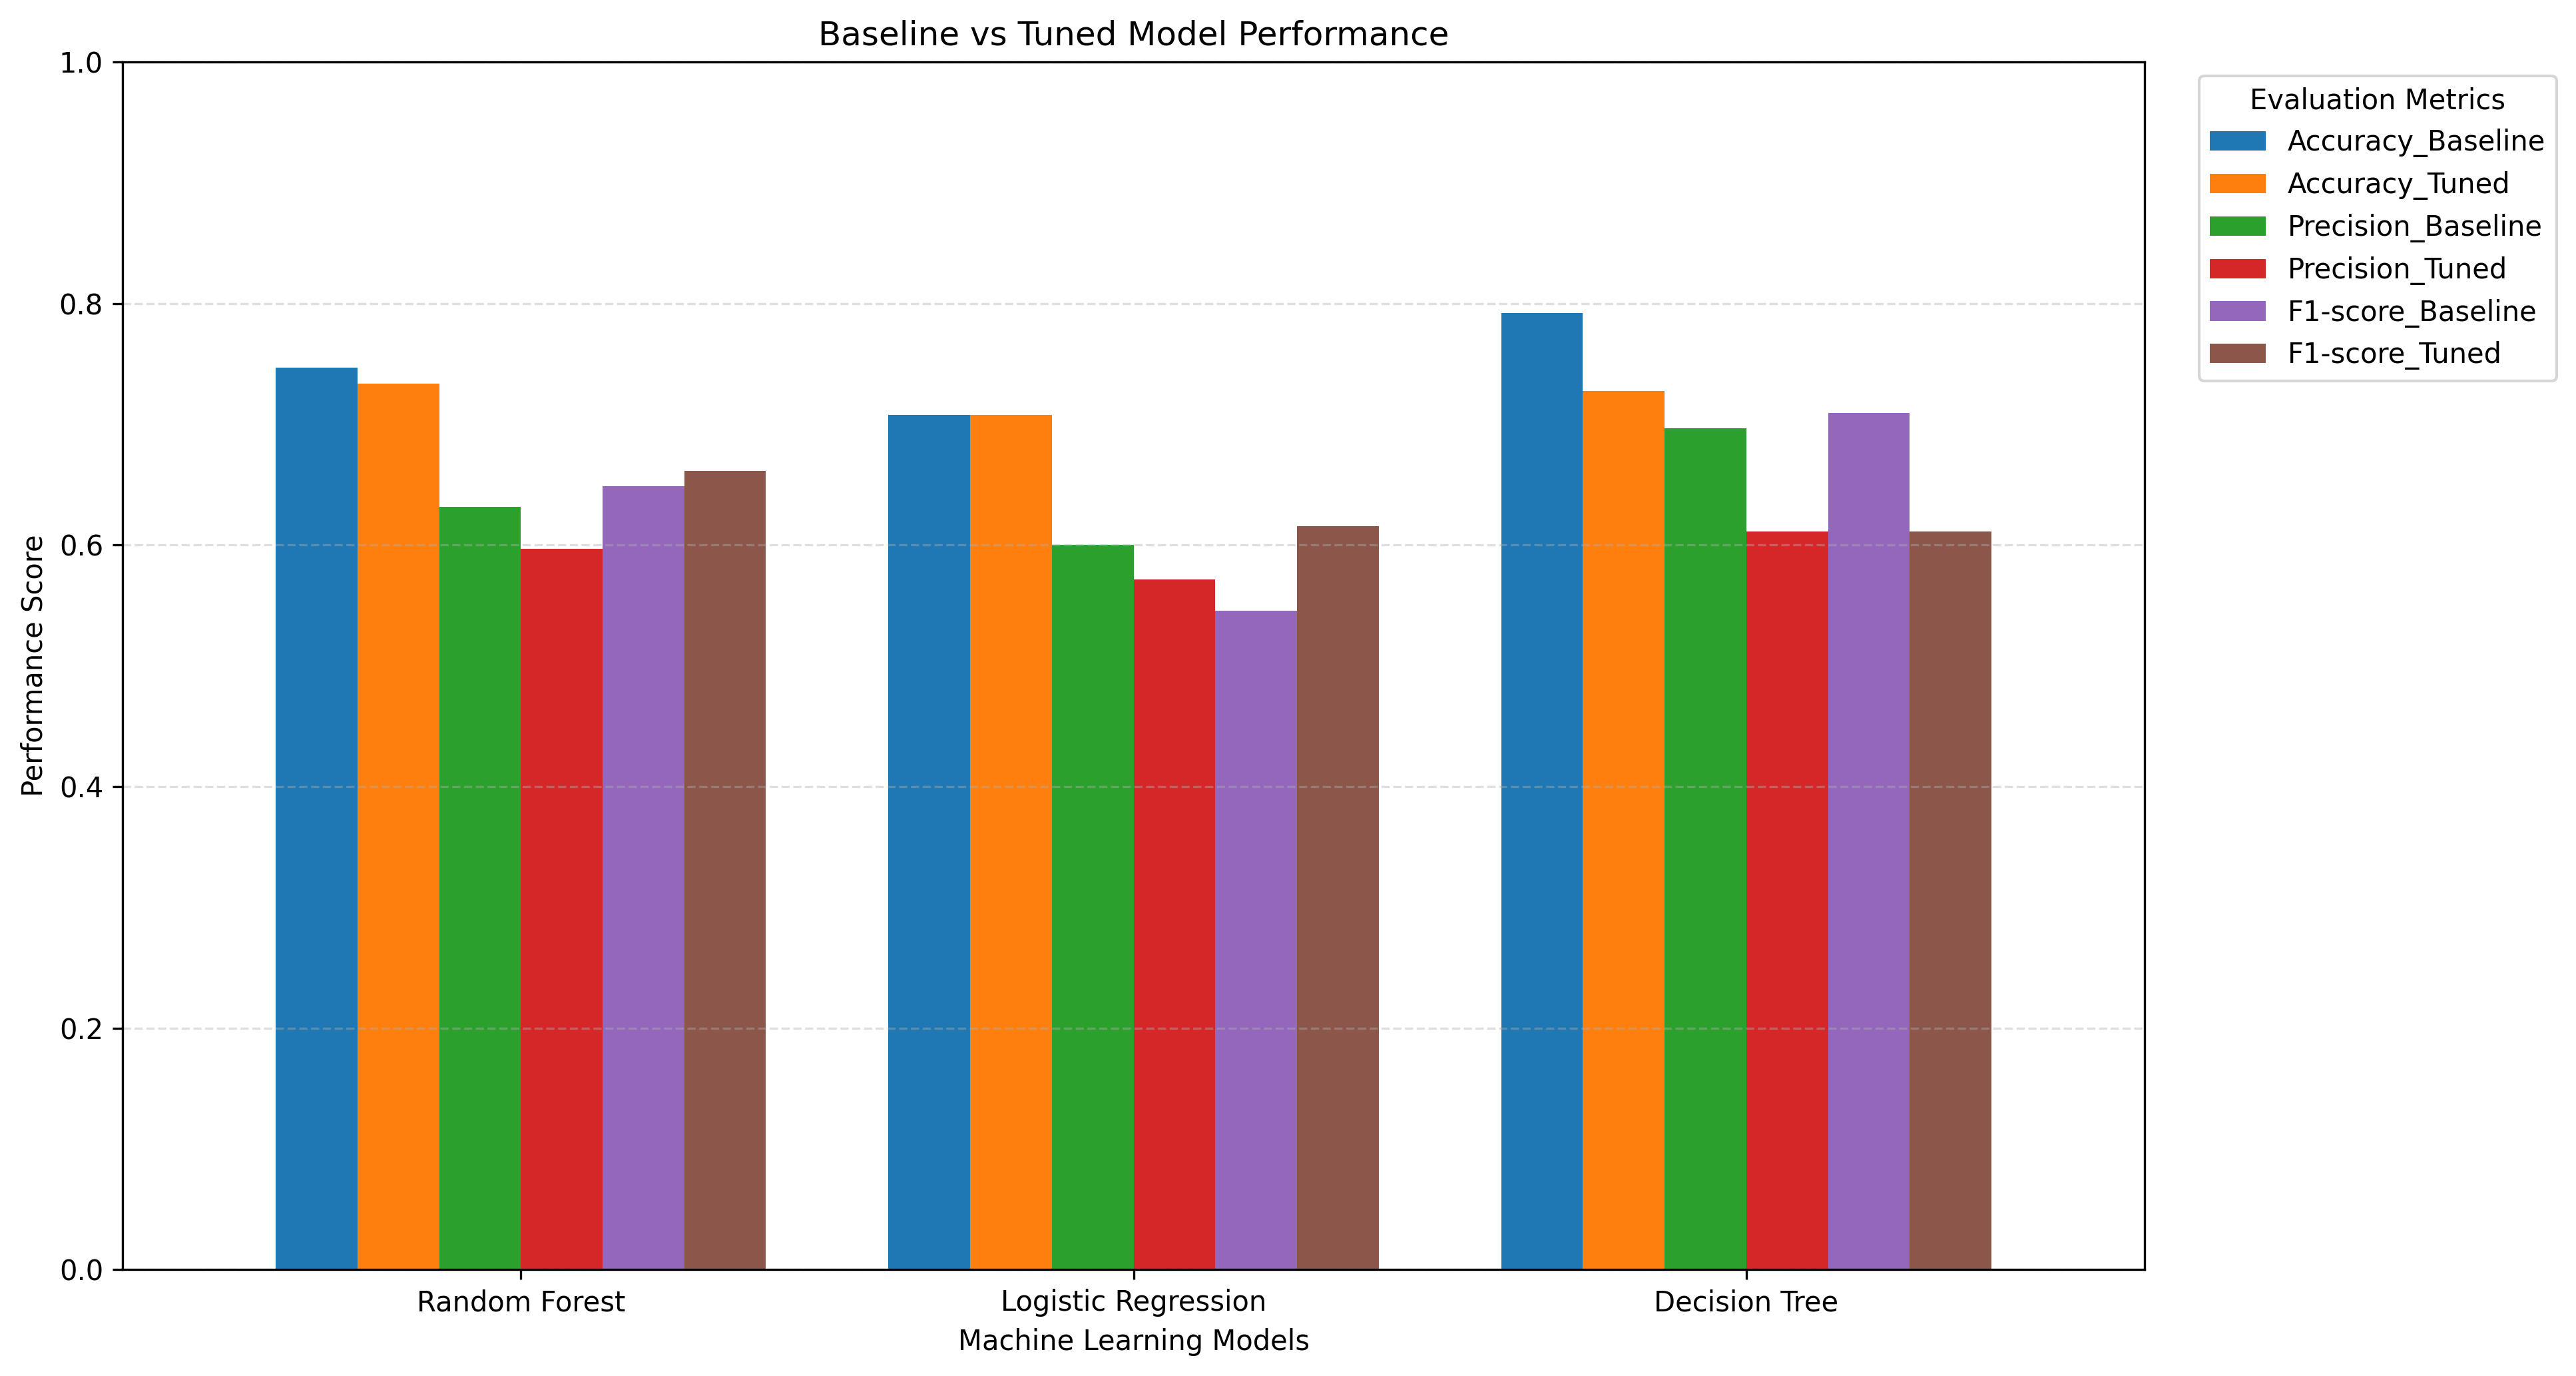
\includegraphics[width=\columnwidth]{figures/baseline_tuned_comparison.png}
\caption{Comparison of baseline and tuned model accuracy, precision, and F1-score.}
\label{fig:comparison}
\end{figure}

\subsection{Feature Selection}
The five selected features were Glucose, SkinThickness, Insulin, BMI, and Age. Compared with all eight features, the selected-feature Random Forest achieved test accuracy of 0.753, recall of 0.759, F1-score of 0.683, and ROC-AUC of 0.819. Logistic Regression achieved accuracy of 0.721 and ROC-AUC of 0.787 with five features, compared with 0.708 and 0.813 using all eight. Decision Tree accuracy and F1-score remained unchanged at 0.792 and 0.709, while ROC-AUC increased from 0.801 to 0.809. Feature reduction therefore had model-dependent effects.

\begin{table}[t]
\caption{Performance With All Eight and Selected Five Features}
\label{tab:featureselection}
\centering
\begin{tabular}{lcccc}
\toprule
& \multicolumn{2}{c}{Accuracy} & \multicolumn{2}{c}{ROC-AUC}\\
Model & 8 feat. & 5 feat. & 8 feat. & 5 feat.\\
\midrule
Logistic Regression & 0.708 & 0.721 & 0.813 & 0.787\\
Decision Tree & 0.792 & 0.792 & 0.801 & 0.809\\
Random Forest & 0.747 & 0.753 & 0.817 & 0.819\\
\bottomrule
\end{tabular}
\end{table}

\subsection{Permutation Feature Importance}
Permutation importance was calculated for the baseline Random Forest, selected because it had the highest baseline test ROC-AUC. Glucose had the largest mean importance (0.1077), followed by BMI (0.0405) and Age (0.0240). The remaining mean importance values were considerably smaller. SkinThickness and BloodPressure had slightly negative mean values, indicating that shuffling them did not reduce ROC-AUC on average in this test-set analysis.

\begin{figure}[t]
\centering
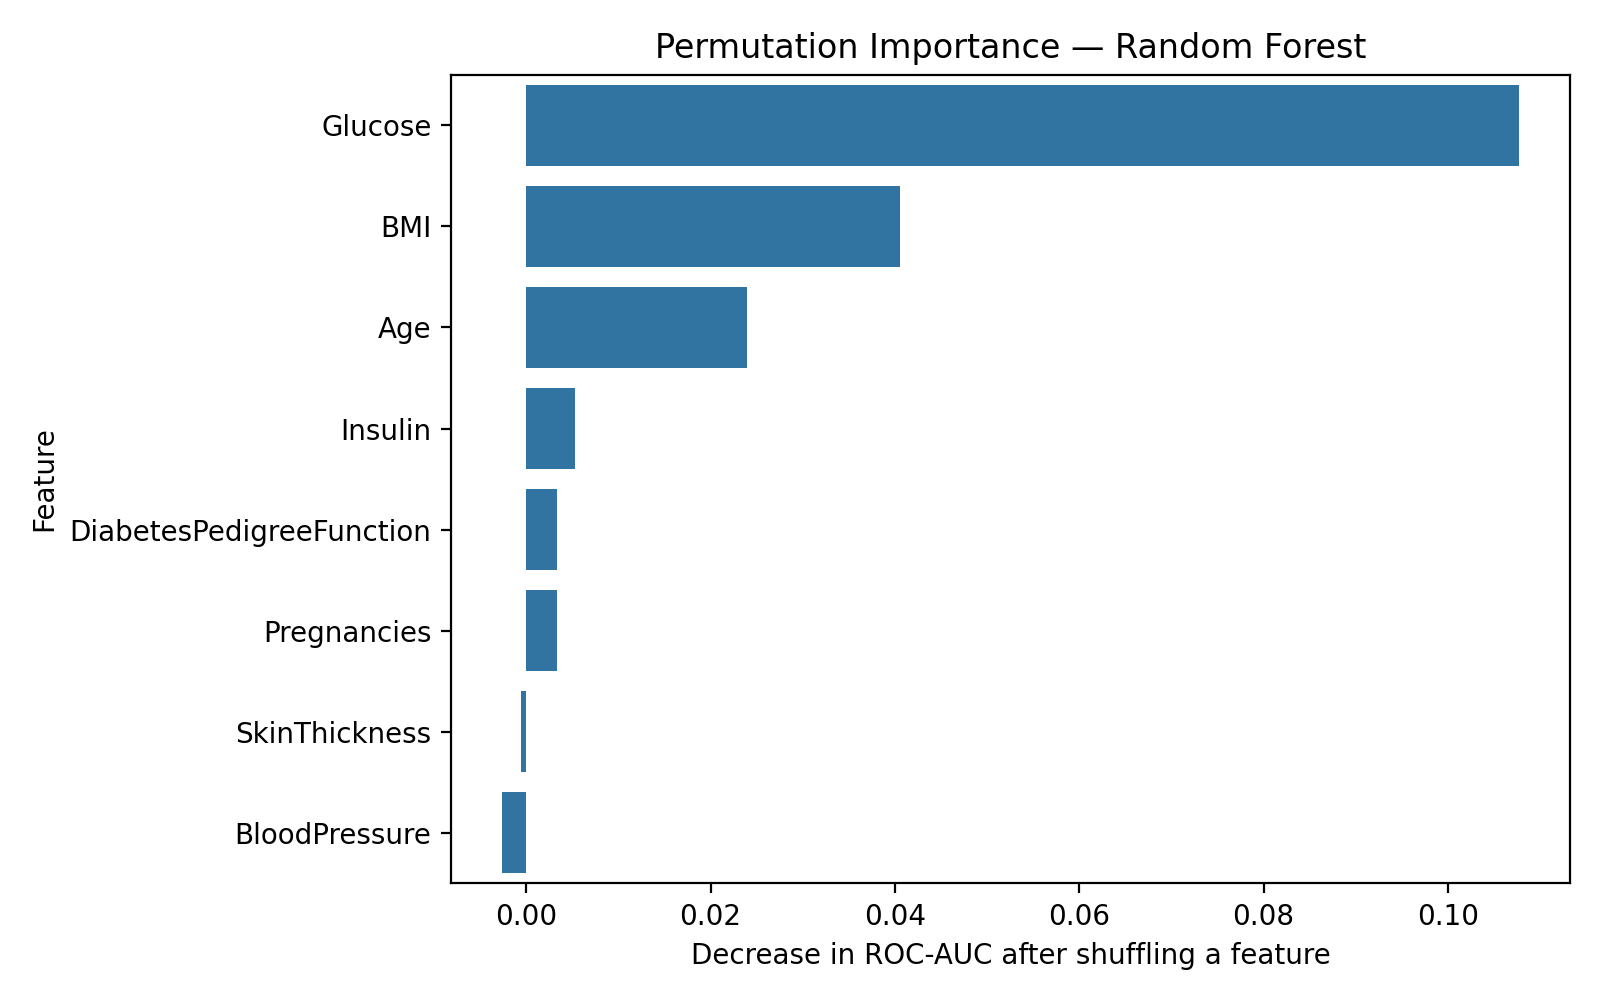
\includegraphics[width=\columnwidth]{figures/permutation_importance.png}
\caption{Permutation importance for the baseline Random Forest model.}
\label{fig:importance}
\end{figure}

\subsection{Five-Fold Cross-Validation}
Five-fold stratified cross-validation was performed on the training data for the baseline pipelines. Logistic Regression achieved the highest mean accuracy (0.788) and ROC-AUC (0.843). Random Forest achieved the highest mean F1-score (0.679) and recall (0.696). Decision Tree had the lowest mean ROC-AUC (0.778). The cross-validation results differ from the single held-out test ranking, reinforcing the need to report both estimates.

\begin{table}[t]
\caption{Five-Fold Cross-Validation Results on Training Data (Mean)}
\label{tab:cv}
\centering
\begin{tabular}{lccccc}
\toprule
Model & Acc. & Prec. & Rec. & F1 & AUC\\
\midrule
Logistic Regression & \textbf{0.788} & \textbf{0.764} & 0.575 & 0.655 & \textbf{0.843}\\
Decision Tree & 0.725 & 0.638 & 0.542 & 0.581 & 0.778\\
Random Forest & 0.770 & 0.665 & \textbf{0.696} & \textbf{0.679} & 0.836\\
\bottomrule
\end{tabular}
\end{table}

\clearpage
\section{Discussion}
The experiments show that model ranking depends on the evaluation metric and validation procedure. The baseline Decision Tree performed best on accuracy and F1-score on the single test split, while baseline Random Forest had the highest test ROC-AUC. Under five-fold cross-validation, Logistic Regression had the highest mean accuracy and ROC-AUC, whereas Random Forest had the highest mean F1-score. This difference is plausible in a relatively small dataset and demonstrates why model selection should not be based on one metric or one split alone.

Hyperparameter tuning was conducted by selecting configurations that maximised cross-validation F1-score. The tuned Random Forest improved test recall and F1-score relative to its baseline counterpart, but its precision and accuracy decreased. The tuned Logistic Regression showed a similar precision--recall trade-off. The tuned Decision Tree did not improve on the test set. These outcomes suggest that the tuning objective changes the operating balance between false positives and false negatives; it does not guarantee a universal improvement.

The feature-selection experiment also produced mixed results. Random Forest showed modest gains in accuracy, recall, F1-score, and ROC-AUC with five features, whereas Logistic Regression's ROC-AUC declined. Decision Tree retained the same accuracy and F1-score. Consequently, the selected five-feature subset may offer a simpler representation for some models, but the experiment does not establish that five features are generally optimal.

Glucose, BMI, and Age were the most influential variables in the baseline Random Forest permutation analysis. These values describe model reliance in this particular dataset and test split. They should not be interpreted as causal effects or as a clinical ranking of risk factors.

\clearpage
\section{Limitations}
Several limitations should be considered:
\begin{itemize}
    \item The dataset contains 768 observations and represents a restricted population of adult women of Pima heritage. Results cannot be assumed to generalise to other populations.
    \item The binary target represents recorded diabetes status. The available file does not provide longitudinal onset times, so the study does not validate prospective prediction before disease onset.
    \item A single stratified 80:20 split was used for the final test evaluation. Repeated nested cross-validation or external validation would provide stronger evidence of generalisation.
    \item The test set was used for descriptive permutation importance and feature-selection comparison, so these analyses should be treated as exploratory rather than independent confirmatory evidence.
    \item No probability calibration, decision-curve analysis, external clinical validation, or prospective evaluation was conducted.
    \item The study is an educational machine-learning experiment and is not a clinically validated diagnostic system.
\end{itemize}

\clearpage
\section{Conclusion and Future Work}
This study compared Logistic Regression, Decision Tree, and Random Forest models for diabetes status prediction using the Pima Indians Diabetes dataset. The baseline Decision Tree achieved the highest test accuracy (79.2\%) and F1-score (70.9\%), while baseline Random Forest achieved the highest test ROC-AUC (0.817). After hyperparameter tuning, Random Forest achieved the highest tuned test recall (74.1\%) and F1-score (66.1\%). Feature selection produced mixed, model-dependent changes, and permutation importance identified Glucose, BMI, and Age as the leading features for the baseline Random Forest.

Future work should evaluate the workflow using larger and more diverse datasets, repeated or nested cross-validation, and independent external test cohorts. Further work could examine calibration, threshold selection, fairness across demographic groups, and clinically relevant decision metrics. Longitudinal data with clearly defined prediction horizons would be required to investigate prediction of future diabetes onset rather than classification of an existing status label.

\clearpage
\section*{Acknowledgment}
The authors may add acknowledgments, institutional support, or project supervision details here, if applicable.

\clearpage
\bibliographystyle{IEEEtran}
\bibliography{references}

\end{document}
